% Options for packages loaded elsewhere
% Options for packages loaded elsewhere
\PassOptionsToPackage{unicode}{hyperref}
\PassOptionsToPackage{hyphens}{url}
\PassOptionsToPackage{dvipsnames,svgnames,x11names}{xcolor}
%
\documentclass[
]{interact}
\usepackage{xcolor}
\usepackage{amsmath,amssymb}
\setcounter{secnumdepth}{5}
\usepackage{iftex}
\ifPDFTeX
  \usepackage[T1]{fontenc}
  \usepackage[utf8]{inputenc}
  \usepackage{textcomp} % provide euro and other symbols
\else % if luatex or xetex
  \usepackage{unicode-math} % this also loads fontspec
  \defaultfontfeatures{Scale=MatchLowercase}
  \defaultfontfeatures[\rmfamily]{Ligatures=TeX,Scale=1}
\fi
\usepackage{lmodern}
\ifPDFTeX\else
  % xetex/luatex font selection
\fi
% Use upquote if available, for straight quotes in verbatim environments
\IfFileExists{upquote.sty}{\usepackage{upquote}}{}
\IfFileExists{microtype.sty}{% use microtype if available
  \usepackage[]{microtype}
  \UseMicrotypeSet[protrusion]{basicmath} % disable protrusion for tt fonts
}{}
\makeatletter
\@ifundefined{KOMAClassName}{% if non-KOMA class
  \IfFileExists{parskip.sty}{%
    \usepackage{parskip}
  }{% else
    \setlength{\parindent}{0pt}
    \setlength{\parskip}{6pt plus 2pt minus 1pt}}
}{% if KOMA class
  \KOMAoptions{parskip=half}}
\makeatother
% Make \paragraph and \subparagraph free-standing
\makeatletter
\ifx\paragraph\undefined\else
  \let\oldparagraph\paragraph
  \renewcommand{\paragraph}{
    \@ifstar
      \xxxParagraphStar
      \xxxParagraphNoStar
  }
  \newcommand{\xxxParagraphStar}[1]{\oldparagraph*{#1}\mbox{}}
  \newcommand{\xxxParagraphNoStar}[1]{\oldparagraph{#1}\mbox{}}
\fi
\ifx\subparagraph\undefined\else
  \let\oldsubparagraph\subparagraph
  \renewcommand{\subparagraph}{
    \@ifstar
      \xxxSubParagraphStar
      \xxxSubParagraphNoStar
  }
  \newcommand{\xxxSubParagraphStar}[1]{\oldsubparagraph*{#1}\mbox{}}
  \newcommand{\xxxSubParagraphNoStar}[1]{\oldsubparagraph{#1}\mbox{}}
\fi
\makeatother


\usepackage{longtable,booktabs,array}
\usepackage{calc} % for calculating minipage widths
% Correct order of tables after \paragraph or \subparagraph
\usepackage{etoolbox}
\makeatletter
\patchcmd\longtable{\par}{\if@noskipsec\mbox{}\fi\par}{}{}
\makeatother
% Allow footnotes in longtable head/foot
\IfFileExists{footnotehyper.sty}{\usepackage{footnotehyper}}{\usepackage{footnote}}
\makesavenoteenv{longtable}
\usepackage{graphicx}
\makeatletter
\newsavebox\pandoc@box
\newcommand*\pandocbounded[1]{% scales image to fit in text height/width
  \sbox\pandoc@box{#1}%
  \Gscale@div\@tempa{\textheight}{\dimexpr\ht\pandoc@box+\dp\pandoc@box\relax}%
  \Gscale@div\@tempb{\linewidth}{\wd\pandoc@box}%
  \ifdim\@tempb\p@<\@tempa\p@\let\@tempa\@tempb\fi% select the smaller of both
  \ifdim\@tempa\p@<\p@\scalebox{\@tempa}{\usebox\pandoc@box}%
  \else\usebox{\pandoc@box}%
  \fi%
}
% Set default figure placement to htbp
\def\fps@figure{htbp}
\makeatother


% definitions for citeproc citations
\NewDocumentCommand\citeproctext{}{}
\NewDocumentCommand\citeproc{mm}{%
  \begingroup\def\citeproctext{#2}\cite{#1}\endgroup}
\makeatletter
 % allow citations to break across lines
 \let\@cite@ofmt\@firstofone
 % avoid brackets around text for \cite:
 \def\@biblabel#1{}
 \def\@cite#1#2{{#1\if@tempswa , #2\fi}}
\makeatother
\newlength{\cslhangindent}
\setlength{\cslhangindent}{1.5em}
\newlength{\csllabelwidth}
\setlength{\csllabelwidth}{3em}
\newenvironment{CSLReferences}[2] % #1 hanging-indent, #2 entry-spacing
 {\begin{list}{}{%
  \setlength{\itemindent}{0pt}
  \setlength{\leftmargin}{0pt}
  \setlength{\parsep}{0pt}
  % turn on hanging indent if param 1 is 1
  \ifodd #1
   \setlength{\leftmargin}{\cslhangindent}
   \setlength{\itemindent}{-1\cslhangindent}
  \fi
  % set entry spacing
  \setlength{\itemsep}{#2\baselineskip}}}
 {\end{list}}
\usepackage{calc}
\newcommand{\CSLBlock}[1]{\hfill\break\parbox[t]{\linewidth}{\strut\ignorespaces#1\strut}}
\newcommand{\CSLLeftMargin}[1]{\parbox[t]{\csllabelwidth}{\strut#1\strut}}
\newcommand{\CSLRightInline}[1]{\parbox[t]{\linewidth - \csllabelwidth}{\strut#1\strut}}
\newcommand{\CSLIndent}[1]{\hspace{\cslhangindent}#1}



\setlength{\emergencystretch}{3em} % prevent overfull lines

\providecommand{\tightlist}{%
  \setlength{\itemsep}{0pt}\setlength{\parskip}{0pt}}



 


\usepackage{booktabs}
\usepackage{longtable}
\usepackage{array}
\usepackage{multirow}
\usepackage{wrapfig}
\usepackage{float}
\usepackage{colortbl}
\usepackage{pdflscape}
\usepackage{tabu}
\usepackage{threeparttable}
\usepackage{threeparttablex}
\usepackage[normalem]{ulem}
\usepackage{makecell}
\usepackage{xcolor}
\usepackage{orcidlink}
\makeatletter
\@ifpackageloaded{caption}{}{\usepackage{caption}}
\AtBeginDocument{%
\ifdefined\contentsname
  \renewcommand*\contentsname{Table of contents}
\else
  \newcommand\contentsname{Table of contents}
\fi
\ifdefined\listfigurename
  \renewcommand*\listfigurename{List of Figures}
\else
  \newcommand\listfigurename{List of Figures}
\fi
\ifdefined\listtablename
  \renewcommand*\listtablename{List of Tables}
\else
  \newcommand\listtablename{List of Tables}
\fi
\ifdefined\figurename
  \renewcommand*\figurename{Figure}
\else
  \newcommand\figurename{Figure}
\fi
\ifdefined\tablename
  \renewcommand*\tablename{Table}
\else
  \newcommand\tablename{Table}
\fi
}
\@ifpackageloaded{float}{}{\usepackage{float}}
\floatstyle{ruled}
\@ifundefined{c@chapter}{\newfloat{codelisting}{h}{lop}}{\newfloat{codelisting}{h}{lop}[chapter]}
\floatname{codelisting}{Listing}
\newcommand*\listoflistings{\listof{codelisting}{List of Listings}}
\makeatother
\makeatletter
\makeatother
\makeatletter
\@ifpackageloaded{caption}{}{\usepackage{caption}}
\@ifpackageloaded{subcaption}{}{\usepackage{subcaption}}
\makeatother
\usepackage{bookmark}
\IfFileExists{xurl.sty}{\usepackage{xurl}}{} % add URL line breaks if available
\urlstyle{same}
\hypersetup{
  pdftitle={Dampak Tarif Resiprokal Trump Terhadap Perekonomian Indonesia: GTAP Model},
  pdfauthor={Krisna Gupta; Arief Anshory Yusuf; M. Hafizh Ghifari Azizi; Shakuntala Anjani Nindraswari},
  pdfkeywords={GTAP, Tarif resiprokal, Dampak ekonomi},
  colorlinks=true,
  linkcolor={blue},
  filecolor={Maroon},
  citecolor={Blue},
  urlcolor={Blue},
  pdfcreator={LaTeX via pandoc}}


\title{Dampak Tarif Resiprokal Trump Terhadap Perekonomian Indonesia:
GTAP Model}
\author{Krisna
Gupta$\textsuperscript{1}$~\orcidlink{0000-0001-8695-0514}, Arief
Anshory Yusuf$\textsuperscript{1}$, M. Hafizh Ghifari
Azizi$\textsuperscript{1}$, Shakuntala Anjani
Nindraswari$\textsuperscript{1}$}

\thanks{CONTACT: Krisna
Gupta. Email: \href{mailto:krisna@dewanekonomi.go.id}{\nolinkurl{krisna@dewanekonomi.go.id}}. }
\begin{document}
\captionsetup{labelsep=space}
\maketitle
\textsuperscript{1}  National Economic Council, Republic of
Indonesia, Jakarta, Indonesia
\begin{abstract}
``Laporan ini merupakan hasil simulasi GTAP versi 7 untuk skenario tarif
Trump untuk Indonesia.''
\end{abstract}
\begin{keywords}
\def\sep{;\ }
GTAP\sep Tarif resiprokal\sep 
Dampak ekonomi
\end{keywords}


\section{Introduction}\label{introduction}

Pada 2 April 2025, Presiden Amerika Serikat Donald J. Trump
mendeklarasikan ``Liberation Day'' setelah sebelumnya menandatangani
memorandum terkait kebijakan perdagangan untuk menyelidiki defisit
perdagangan AS dan praktik tidak adil mitra dagang AS. Presiden Trump
menilai adanya ketimpangan tarif dan hambatan non tarif, serta kebijakan
ekonomi sejumlah mitra dagang yang menekan tingkat upah dan konsumsi
domestik telah berkontribusi pada defisit perdagangan tahunan yang besar
dan berkelanjutan bagi Amerika Serikat. Hal ini dianggap oleh Presiden
Trump suatu ancaman terhadap keamanan nasional dan stabilitas
perekonomian nasional.

Pada hari tersebut, Presiden Trump mengumumkan tarif dalam dua tingkat:
tarif baseline sebesar 10\% yang dikenakan pada impor dari semua negara
yang tidak dikenai sanksi lain serta tarif tambahan setiap negara yang
disebut tarif resiprokal yang berkisar antara 11\% hingga 50\% bagi
negara-negara tertentu, termasuk terhadap negara-negara ASEAN seperti
Vietnam (46\%), Thailand (36\%), Indonesia (32\%), dikenakan tarif yang
secara relatif lebih besar dibandingkan negara lainnya, seperti India
(27\%), Korea Selatan (26\%), Jepang (24\%), dan Uni Eropa (20\%) (The
White House 2025).

Laporan ini bertujuan untuk menganalisis dampak kebijakan tarif
resiprokal AS terhadap perekonomian Indonesia, termasuk dampaknya
terhadap PDB, neraca perdagangan, ekspor, impor, inflasi, kesejahteraan,
dan ketenagakerjaan. paper ini diharapkan memberikan sumbangan terhadap
literatur perdagangan internasional kontemporer melalui penyajian
analisis dalam kerangka multi-negara. Selain itu, makalah ini turut
memperkaya literatur mengenai tarif resiprokal dengan menunjukkan adanya
pola dampak yang serupa sebagaimana teridentifikasi dalam isu tersebut.

Simulasi dilakukan dengan model standar GTAP versi 7 (Corong et al.
2017) dan GTAP database versi 11 (Aguiar et al. 2022). Tidak ada
modifikasi pada model maupun database yang dilakukan di dalam simulasi
ini.

\section{Dinamika Tarif Resiprokal
AS}\label{dinamika-tarif-resiprokal-as}

Terdapat beberapa tahap perubahan besaran tarif resiprokal AS terhadap
berbagai negara, termasuk Indonesia. Saat pengumuman tarif tahap 1 pada
2 April 2025, AS mengenakan tarif resiprokal 32\% terhadap seluruh
barang Indonesia. Pemerintah merespon cepat atas pengenaan tarif yang
relatif tinggi tersebut dan melakukan negosiasi melalui beberapa
penawaran seperti penghapusan sebagian atau seluruh barang AS,
penghapusan NTB (Non-Tariff Barriers), dan juga rencana peningkatan
investasi ke AS.

Hal ini menghasilkan kesepakatan bahwa AS akan menurunkan besaran tarif
resiprokalnya terhadap Indonesia menjadi 19\% atau yang terendah
diantara negara ASEAN lainnya sebelum akhirnya AS pun menurunkan tarif
resiprokalnya terhadap negara-negara lainnya, termasuk Vietnam menjadi
20\% dan Cambodia, Thailand, Malaysia, Philippines menjadi 19\% pada 31
Juli 2025. Selain itu, beberapa negara/kawasan lainnya juga mendapatkan
tarif lebih rendah dibandingkan Indonesia seperti Korea Selatan, Jepang,
dan Uni Eropa, yakni sebesar 15\%.

\begin{longtable}[]{@{}
  >{\raggedleft\arraybackslash}p{(\linewidth - 10\tabcolsep) * \real{0.0348}}
  >{\raggedright\arraybackslash}p{(\linewidth - 10\tabcolsep) * \real{0.0435}}
  >{\raggedright\arraybackslash}p{(\linewidth - 10\tabcolsep) * \real{0.2783}}
  >{\raggedleft\arraybackslash}p{(\linewidth - 10\tabcolsep) * \real{0.2174}}
  >{\raggedleft\arraybackslash}p{(\linewidth - 10\tabcolsep) * \real{0.2174}}
  >{\raggedleft\arraybackslash}p{(\linewidth - 10\tabcolsep) * \real{0.2087}}@{}}

\caption{\label{tbl-tarif}Dinamika tarif resiprokal AS terhadap berbagai
negara}

\tabularnewline

\toprule\noalign{}
\begin{minipage}[b]{\linewidth}\raggedleft
No.
\end{minipage} & \begin{minipage}[b]{\linewidth}\raggedright
Code
\end{minipage} & \begin{minipage}[b]{\linewidth}\raggedright
Description
\end{minipage} & \begin{minipage}[b]{\linewidth}\raggedleft
Tarif 1 (Sampai 2 April)
\end{minipage} & \begin{minipage}[b]{\linewidth}\raggedleft
Tarif 2 (Sampai 31 Juli)
\end{minipage} & \begin{minipage}[b]{\linewidth}\raggedleft
Tarif 3 (Sampai 16 Sep)
\end{minipage} \\
\midrule\noalign{}
\endhead
\bottomrule\noalign{}
\endlastfoot
1 & chn & China & 0.55 & 0.55 & 0.55 \\
2 & ind & India & 0.26 & 0.25 & 0.50 \\
3 & lao & Lao People's Democratic Republ & 0.48 & 0.40 & 0.40 \\
4 & can & Canada & 0.25 & 0.35 & 0.35 \\
5 & zaf & South Africa & 0.30 & 0.30 & 0.30 \\
6 & mex & Mexico & 0.25 & 0.30 & 0.30 \\
7 & brn & Brunei Darussalam & 0.24 & 0.25 & 0.25 \\
8 & vnm & Viet Nam & 0.46 & 0.20 & 0.20 \\
9 & khm & Cambodia & 0.49 & 0.19 & 0.19 \\
10 & tha & Thailand & 0.36 & 0.19 & 0.19 \\
11 & idn & Indonesia & 0.32 & 0.19 & 0.19 \\
12 & mys & Malaysia & 0.24 & 0.19 & 0.19 \\
13 & phl & Philippines & 0.17 & 0.19 & 0.19 \\
14 & kor & Republic of Korea & 0.25 & 0.15 & 0.15 \\
15 & jpn & Japan & 0.24 & 0.15 & 0.15 \\
16 & fra & France & 0.20 & 0.15 & 0.15 \\
17 & deu & Germany & 0.20 & 0.15 & 0.15 \\
18 & ita & Italy & 0.20 & 0.15 & 0.15 \\
19 & eu & European Union & 0.20 & 0.15 & 0.15 \\
20 & tur & Turkiye & 0.10 & 0.15 & 0.15 \\
21 & arg & Argentina & 0.10 & 0.10 & 0.10 \\
22 & aus & Australia & 0.10 & 0.10 & 0.10 \\
23 & bra & Brazil & 0.10 & 0.10 & 0.10 \\
24 & rus & Russian Federation & 0.10 & 0.10 & 0.10 \\
25 & sau & Saudi Arabia & 0.10 & 0.10 & 0.10 \\
26 & sgp & Singapore & 0.10 & 0.10 & 0.10 \\
27 & gbr & United Kingdom of Great Britain & 0.10 & 0.10 & 0.10 \\

\end{longtable}

Pada 27 Agustus 2025, AS kembali menaikan tarif resiprokal pada India
menjadi 50\% meskipun sebelumnya AS memotong 1\% poin tarif
resiprokalnya terhadap India. Kebijakan ini diklaim sebagai hukuman
terhadap India atas pembelian minyak dan senjata dari Rusia yang dinilai
membantu mendanai perangnya dengan Ukraina.

\section{Perdagangan Bilateral Indonesia -- Amerika
Serikat}\label{perdagangan-bilateral-indonesia-amerika-serikat}

Amerika Serikat merupakan salah satu mitra dagang penting bagi Indonesia
yang. Pada tahun 2024, AS menjadi negara penyumbang surplus neraca
perdagangan terbesar, yaitu sebesar USD14,4 miliar. Pangsa pasar AS bagi
ekspor Indonesia sebesar USD26,4 miliar atau 10,6\% total ekspor
nasional, menjadi yang terbesar kedua setelah China yang memiliki pangsa
USD60,2 miliar atau 24,2\%. Selain itu, komoditas ekspor Indonesia ke AS
mayoritas merupakan sektor padat karya dengan AS sebagai negara tujuan
utama ekspor seperti komoditas tekstil dan produk tekstil (55,4\%), alas
kaki (33,8\%), furnitur (59,1\%), dan komoditas perikanan dan udang
(35,0\%).

Tarif resiprokal 32\% berpotensi menurunkan daya saing ekspor Indonesia
secara signifikan, terutama jika negara kompetitor memiliki tarif yang
jauh lebih rendah. Hal ini dapat terlihat pada sektor udang dan
perikanan, di mana ekuador menjadi kompetitor Indonesia yang kuat dengan
volume produksi yang tinggi, beban tarif yang lebih rendah (10\%), dan
jarak geografis yang lebih dekat ke AS.

Penurunan tarif AS terhadap Indonesia dari 32\% menjadi 19\% dapat
terlihat dari posisi Indonesia yang menjadi lebih kompetitif
dibandingkan dengan tarif yang diumumkan pada Presiden Trump pada 2
April 2025. Jika dilihat dari produk-produk ekspor utama Indonesia ke
AS, seperti alas kaki, pakaian dan aksesoris pakaian, lemak dan minyak
hewan/nabati, karet, serta olahan daging dan ikan, Indonesia menempati
peringkat dengan tarif yang relatif lebih rendah dibandingkan
negara-negara kompetitor lainnya, termasuk Vietnam, Bangladesh, dan
India.

Di sisi lain, Indonesia mengimpor USD12,0 miliar barang dari AS atau
5,1\% dari total impor nasional 2024 dan menjadi terbesar ke-4 setelah
China (31,1\%), Singapura (9,2\%), dan Jepang (6,4\%). Adapun komoditas
impor utama indonesia dari AS adalah bahan bakar mineral \& minyak bumi
(24,4\%), mesin \& peralatan mekanik (12,6\%), minyak biji-bijian \&
hasil pertanian (10,5\%), limbah industri makanan \& pakan ternak
(5,4\%), dan mesin listrik \& peralatan elektronik (4,1\%).

\section{Metode}\label{metode}

\subsection{GTAP Model}\label{gtap-model}

GTAP versi 7 merupakan sebuah model riil dengna multi-sektor dan
multi-regional. Setiap negara terdiri dari 1 rumah tangga representatif
yang melakukan konsumsi privat (\emph{private consumption, C}), menabung
(sehingga memberi suplai permodalan), dan faktor produksi (tenaga kerja,
tepatnya). Tabungan tersebut dipool ke dalam sebuah bank yang kemudian
mendistribusikannya ke berbagai sektor.

Setiap negara memiliki berbagai sektor yang diwakili 1 perusahaan yang
mengambil tenaga kerja dan investasi dari rumah tangga dan bank. Setiap
sektor juga mengambil input dari sektor lain.

Rumah tangga dan industri membeli barang dan jasa dari sektor industri
domestik maupun impor. Produk domestik dan impor dapat saling
menggantikan dengan sebuah elastisitas bernama elastisitas Armington.
Pendekatan ini adalah pendekatan standar dalam analisis perdagangan
internasional.

\subsection{Closure dan shock}\label{closure-dan-shock}

Simulasi ini menggunakan \emph{unemployment closure} di mana kami
melakukan \emph{swap} antara real wage labor supply, yang seringkali
disebut juga sebagai \emph{sticky wage closure}. \emph{sticky wage}
berarti upahnya tidak bergerak. Ada perpindahan pekerja antar-sektor,
tapi total employment berubah (bisa berkurang, bisa bertambah). Pada
kenyataannya, upah mungkin saja tidak sepenuhnya sticky.

Semua simulasi tersebut dilakukan dengan situasi di mana Vietnam terkena
tarif 20\% dan memberikan konsesi 0\% untuk AS. Semua simulasi ketika
Indonesia terkena 19\% tarif AS juga disertai dengan tarif 0\% dari AS
ke Indonesia.

\section{Hasil umum}\label{hasil-umum}

Beberapa hasil simulasi yang disampaikan di sini adalah hasil makro dan
hasil sektoral.

\begin{figure}

\centering{

\pandocbounded{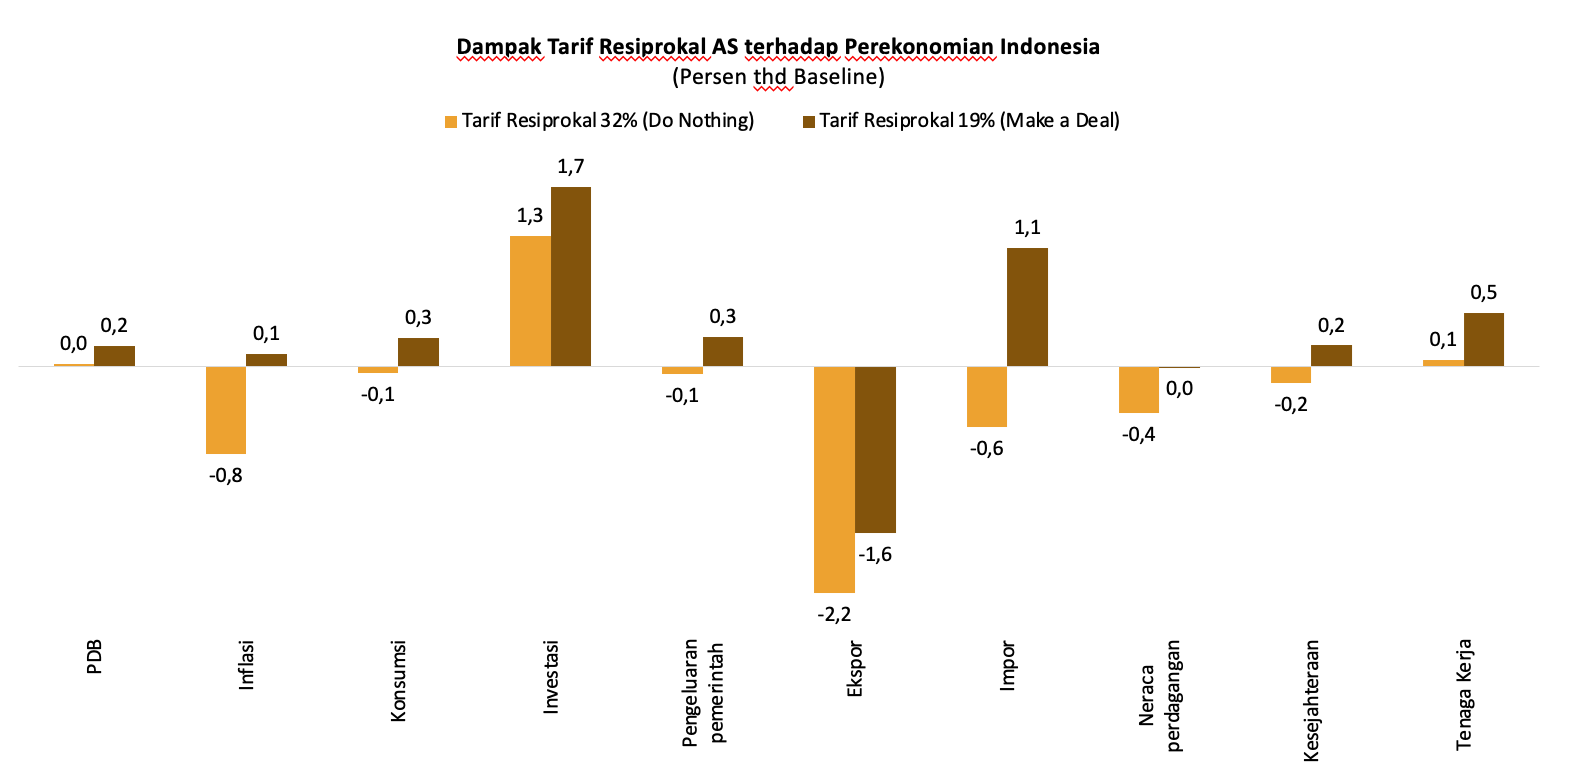
\includegraphics[keepaspectratio]{wew.png}}

}

\caption{\label{fig-1}Dampak tarif resiprokal AS terhadap perekonomian
Indonesia}

\end{figure}%

Hasil makroekonmi dapat dilihat pada Figure~\ref{fig-1}. Hasil GTAP
menunjukan bahwa melakukan negosiasi perdagangan dan mendapatkan tarif
resiprokal yang lebih rendah akan berdampak positif bagi perekonomian
Indonesia. Hal ini dapat dilihat dari beberapa indikator kunci
perekonomian seperti PDB, inflasi, konsumsi masyarakat, investasi,
pengeluaran pemerintah, ekspor impor, neraca perdagangan, kesejahteraan,
maupun ketenagakerjaan.

Turunnya tarif resiprokal terhadap Indonesia menjadi 19\% akan
meningkatkan perubahan PDB nasional sebesar 0,2\%, berbeda dengan ketika
Indonesia dikenakan tarif resiprokal 32\% yang relatif tidak berdampak
pada pertumbuhan PDB. Perubahan ini utamanya ditopang oleh dampak
peningkatan konsumsi (0,3\%), investasi (1,7\%), pengeluaran pemerintah
(0,3\%), dan net ekspor (0,0\%) yang lebih tinggi jika dibandingkan
dampak yang dihasilkan dari dikenakannya tarif resiprokal 32\%.

Investasi menjadi komponen dengan perubahan positif tertinggi
dibandingkan dengan Indikator lainnya. Peningkatan investasi utamanya
akibat beralihnya investasi negara lain yang memiliki tarif resiprokal
lebih tinggi dibanding yang dikenakan terhadap Indonesia, khususnya di
sektor yang memiliki ekspor pasar utama di AS. Beberapa contoh negara
tersebut adalah China (55\%), India (50\%), Laos (40\%), dan Bangladesh
(20\%).

Perubahan tarif resiprokal juga berdampak pada membaliknya perubahan
tingkat inflasi dan kesejahteraan nasional menjadi positif. Perubahan
inflasi dan kesejahteraan meningkat akibat perekonomian yang ekspansif
seiring dengan meningkatnya investasi dan produksi nasional. Sementara
itu, tenaga kerja naik lebih signifikan akibat tumbuhnya industri
nasional, khususnya di sektor industri padat tenaga kerja.

\begin{longtable}[]{@{}
  >{\raggedleft\arraybackslash}p{(\linewidth - 8\tabcolsep) * \real{0.0345}}
  >{\raggedright\arraybackslash}p{(\linewidth - 8\tabcolsep) * \real{0.0805}}
  >{\raggedright\arraybackslash}p{(\linewidth - 8\tabcolsep) * \real{0.4023}}
  >{\raggedleft\arraybackslash}p{(\linewidth - 8\tabcolsep) * \real{0.2414}}
  >{\raggedleft\arraybackslash}p{(\linewidth - 8\tabcolsep) * \real{0.2414}}@{}}

\caption{\label{tbl-sektor}Dampak tarif resiprokal terhadap sektor
industri di Indonesia}

\tabularnewline

\toprule\noalign{}
\begin{minipage}[b]{\linewidth}\raggedleft
No
\end{minipage} & \begin{minipage}[b]{\linewidth}\raggedright
Kode
\end{minipage} & \begin{minipage}[b]{\linewidth}\raggedright
Industri
\end{minipage} & \begin{minipage}[b]{\linewidth}\raggedleft
Tarif Resiprokal 32\%
\end{minipage} & \begin{minipage}[b]{\linewidth}\raggedleft
Tarif Resiprokal 19\%
\end{minipage} \\
\midrule\noalign{}
\endhead
\bottomrule\noalign{}
\endlastfoot
1 & lea & Leather products & -4.81 & 5.05 \\
2 & wap & Wearing apparel & -10.55 & 4.60 \\
3 & cns & Construction & 1.16 & 1.55 \\
4 & ele & Computer, electronic and optic & -0.11 & 0.64 \\
5 & frs & Forestry & 0.52 & 0.55 \\
6 & obs & Business services nec & 0.87 & 0.49 \\
7 & ctl & Bovine cattle, sheep and goats & 0.52 & 0.45 \\
8 & p\_c & Petroleum, coal products & 0.42 & 0.43 \\
9 & omt & Meat products nec & 0.20 & 0.40 \\
10 & trd & Trade & 0.23 & 0.40 \\
11 & otp & Transport nec & 0.26 & 0.37 \\
12 & osg & Public Administration & 0.05 & 0.35 \\
13 & hht & Human health and social work & 0.06 & 0.34 \\
14 & afs & Accommodation, Food and service & 0.74 & 0.32 \\
15 & ros & Recreational and other service & 0.07 & 0.32 \\
16 & atp & Air transport & 0.39 & 0.28 \\
17 & ofi & Financial services nec & 0.16 & 0.28 \\
18 & cmn & Communication & 0.20 & 0.27 \\
19 & ins & Insurance & 0.35 & 0.27 \\
20 & edu & Education & 0.08 & 0.25 \\
21 & oap & Animal products nec & 0.10 & 0.24 \\
22 & dwe & Dwellings & -0.08 & 0.21 \\
23 & wol & Wool, silk-worm cocoons & 0.01 & 0.21 \\
24 & rsa & Real estate activities & 0.42 & 0.21 \\
25 & pcr & Processed rice & 0.07 & 0.19 \\
26 & rmk & Raw milk & 0.27 & 0.19 \\
27 & cmt & Bovine meat products & 0.08 & 0.16 \\
28 & wtr & Water & -0.06 & 0.16 \\
29 & whs & Warehousing and support activities & 0.33 & 0.15 \\
30 & pfb & Plant-based fibers & 1.13 & 0.14 \\
31 & mvh & Motor vehicles and parts & 2.40 & 0.13 \\
32 & nmm & Mineral products nec & 0.33 & 0.12 \\
33 & b\_t & Beverages and tobacco products & 0.05 & 0.10 \\
34 & sgr & Sugar & 0.60 & 0.05 \\
35 & c\_b & Sugar cane, sugar beet & 0.57 & 0.04 \\
36 & pdr & Paddy rice & -0.14 & 0.01 \\
37 & mil & Dairy products & 0.60 & -0.01 \\
38 & otn & Transport equipment nec & 2.37 & -0.07 \\
39 & ome & Machinery and equipment & 2.08 & -0.09 \\
40 & oxt & Minerals nec & 0.65 & -0.10 \\
41 & fsh & Fishing & -0.22 & -0.12 \\
42 & v\_f & Vegetables, fruit, nuts & -0.01 & -0.13 \\
43 & ely & Electricity & -0.36 & -0.21 \\
44 & gdt & Gas manufacture, distribution & -0.57 & -0.38 \\
45 & gro & Cereal grains nec & -0.77 & -0.40 \\
46 & fmp & Metal products & 0.06 & -0.45 \\
47 & wtp & Water transport & -0.16 & -0.49 \\
48 & bph & Basic pharmaceutical products & 1.14 & -0.49 \\
49 & coa & Coal & -0.17 & -0.65 \\
50 & ppp & Paper products, publishing & 0.29 & -0.73 \\
51 & osd & Oil seeds & 0.40 & -0.87 \\
52 & ofd & Food products nec & -1.54 & -0.89 \\
53 & oilgas & Oil \& gas & -0.48 & -1.04 \\
54 & lum & Wood products & -0.76 & -1.04 \\
55 & vol & Vegetable oils and fats & -0.06 & -1.72 \\
56 & ocr & Crops nec & -2.64 & -1.84 \\
57 & eeq & Electrical equipment & -1.18 & -2.15 \\
58 & i\_s & Ferrous metals & 0.27 & -2.17 \\
59 & chm & Chemical products & 0.40 & -2.43 \\
60 & wht & Wheat & -1.26 & -2.59 \\
61 & nfm & Metals nec & 1.18 & -2.61 \\
62 & rpp & Rubber and plastic products & -5.17 & -2.74 \\
63 & tex & Textiles & -4.05 & -3.87 \\
64 & omf & Manufactures nec & -9.82 & -4.62 \\

\end{longtable}

Hasil dari sektor industri dapat dilihat pada Table~\ref{tbl-sektor}.
Penurunan tarif resiprokal menjadi 19\% berdampak positif terhadap
mayoritas industri yang berorientasi pada ekspor dengan pangsa pasar
utama AS. Industri produk kulit dan industri pakaian merupakan industri
yang paling diuntungkan akibat perubahan tarif resiprokal. Dampak pada
industri produk kulit berbalik menjadi +5,05\% saat tarif resiprokal
19\% dari dampak -4,81\% saat tarif resiprokal 32\%, sementara dampak
pada industri pakaian meningkat menjadi +4,6\% dari yang sebelumnya
-10,55\%. Perubahan positif ini terjadi akibat beralihnya beberapa
produksi industri tersebut dari negara yang terkena tarif resiprokal di
atas 19\% ke Indonesia.

Perubahan ini cukup sensitif terhadap hasil dari simulasi. Ketika Brazil
dan India terkena 50\% tarif, hasil simulasi Indonesia 32\% untuk
Indonesia masih memberikan nilai PDB yang tidak berubah, dibandingkan
ketika negara-negara tersebut terkena tarif yang rendah.

Tarif resiprokal yang dikeluarkan oleh Presiden Amerika Serikat Donald
Trump memberikan guncangan yang cukup besar baik untuk pemerintah negara
lain maupun pelaku bisnis. Tidak hanya tinggi levelnya, tarif tersebut
juga terus mengalami perubahan. Publikasi ini bertujuan untuk memberikan
gambaran mengenai kemungkinan dampaknya pada ekonomi Indonesia.
Berdasarkan temuan di publikasi ini, besaran tarif 19\% akan memberikan
dampak yang lebih baik ketimbang tarif 32\%. Di samping itu, besaran
tarif Indonesia harus diusahakan untuk selalu lebih rendah ketimbang
negara lain. Karena itu, Indonesia perlu senantiasa aktif bernegosiasi
sembari memantau tarif yang diberikan AS kepada mitra dagangnya yang
lain.

Fakta bahwa tarif yang dikenakan oleh Presiden Donald Trump terus
mengalami perubahan harus menjadi pertimbangan bagi tim negosiator. Akan
sulit untuk bernegosiasi apabila kesepakatan yang telah dicapai bisa
dengan mudah diamandemen secara sepihak oleh Amerika Serikat. Negosiator
sebaiknya meminta klausul yang melindungi Indonesia dari perubahan nilai
tarif ataupun hambatan dagang lainnya yang dikeluarkan secara sepihak
oleh AS.

\section{Keterbatasan}\label{keterbatasan}

Untuk menerjemahkan hasil simulasi di GTAP, seorang analis harus
mempertimbangkan desain dari model ini. Asumsi ``ceteris paribus'' harus
ditekankan karena setiap negara pasti akan memberikan reaksi terhadap
potensi \emph{outcome} dari sebuah \emph{shock}. Ada beberapa hal yang
perlu diperhatikan:

\begin{enumerate}
\def\labelenumi{\arabic{enumi}.}
\item
  \textbf{Free flow of labor and capital}. Model GTAP yang standar
  mempertimbangkan bahwa setiap pekerja dan kapital dapat ``pindah
  industri'' dengan mudah. Akibatnya, semua pekerja dan kapital memiliki
  return yang sama. Alias, hanya ada 1 upah dan 1 interest rate yang
  sama untuk semua industri di dalam suatu negara. Pada kenyataannya,
  proses adjustment ini tidak terjadi serta merta (butuh waktu), bahkan
  mungkin untuk faktor produksi yang sangat spesifik, perpindahan
  tersebut tidak dapat terjadi sama sekali.
\item
  \textbf{Zero trade cost} mengakibatkan dampak tarif yang relatif mirip
  meskipun negaranya letaknya cukup jauh. Misalnya, hubungan dagang
  Kanada dengan negara lain meningkat cukup pesat, termasuk dengan
  Indonesia. Karena itu hasil perubahan besar Indonesia-Kanada (dan
  dengan negara-negara lain juga) perlu dilihat dengan hati-hati. Meski
  demikian, hal ini tidak berarti tidak mungkin juga. Apalagi Kanada
  juga sedang menjajaki CEPA dengan Indonesia.
\item
  \textbf{Lack of monetary module}. GTAP adalah model riil yang tidak
  mempertimbangkan adanya pasar moneter. Artinya, tidak ada nilai tukar
  di model GTAP. Sebenarnya nilai tukar dapat di-\emph{proxy} dengan
  \emph{terms of trade}. Akan tetapi, yang terpenting adalah tidak
  adanya mekanisme eksogen untuk mengatur pasar uang. Tidak ada bank
  sentral di model ini yang dapat melakukan \emph{quantitative easing}
  atau \emph{intervensi interest rate} dan menciptakan surat utang. Hal
  ini penting karena kebijakan moneter akan mengubah alur barang dan
  jasa lewat nilai tukar dan neraca finansial. Akan tetapi yang lebih
  penting adalah karena saat ini dunia sedang berada di tengah
  ketidakseimbangan neraca finansial akibat dolar yang tidak hanya
  mendominasi, namun juga dikontrol oleh 1 institusi saja. (not a free
  market)
\item
  \textbf{Bebas dari reaksi pengambil kebijakan}: Model GTAP adalah
  model yang dibuat dengan struktur tertentu yang perlu dibaca dalam
  konteks. Model ini dijalankan dengan asumsi ceteris paribus, yang
  artinya diasumsikan bahwa negara-negara di model ini tidak menambahkan
  kebijakan apapun yang berpotensi mengubah arah perputaran ekonomi
  (misalnya subsidi, hambatan perdagangan tambahan, ataupun kebijakan
  industrial lain).
\end{enumerate}

Mengingat setidaknya empat keterbatasan di atas, laporan ini harus
dibaca dengan hati-hati. Laporan ini saja tidak dapat dijadikan
satu-satunya rujukan ataupun patokan dalam mengambil kebijakan.
Diperlukan beberapa penyesuaian dan tambahan studi baik lapangan maupun
empiris yang lebih kontekstual untuk kasus-kasus tertentu.

Laporan ini masih berupa dokumen berjalan dan akan diperbarui seiring
dengan perkembangan situasi. Kritik dan saran sangat kami harapkan untuk
perbaikan laporan ini di masa mendatang.

\section*{Referensi}\label{referensi}
\addcontentsline{toc}{section}{Referensi}

\phantomsection\label{refs}
\begin{CSLReferences}{1}{1}
\bibitem[\citeproctext]{ref-database}
Aguiar, A, M Chepeliev, Erwin Corong, and Dominique van Der Mensbrugghe.
2022. {``The GTAP Data Base: Version 11.''} Journal Article.
\emph{Journal of Global Economic Analysis} 7 (2): 37.
\url{https://www.jgea.org/ojs/index.php/jgea/article/view/181}.

\bibitem[\citeproctext]{ref-model}
Corong, Erwin L., Thomas W. Hertel, Robert A. McDougall, Marinos E.
Tsigas, and Dominique Van Der Mensbrugghe. 2017. {``The Standard GTAP
Model, Version 7.''} Journal Article. \emph{Journal of Global Economic
Analysis} 2 (1): 120.

\bibitem[\citeproctext]{ref-wh}
The White House. 2025. \emph{Regulating Imports with a Reciprocal Tariff
to Rectify Trade Practices That Contribute to Large and Persistent
Annual United States Goods Trade Deficits}.
\href{https://www.whitehouse.gov/presidential-actions/2025/04/regulating-imports-with-a-reciprocal-tariff-to-rectify-trade-practices-that-contribute-to-large-and-persistent-annual-united-states-goods-trade-deficits/}{Https://www.whitehouse.gov/presidential-actions/2025/04/regulating-imports-with-a-reciprocal-tariff-to-rectify-trade-practices-that-contribute-to-large-and-persistent-annual-united-states-goods-trade-deficits/}.

\end{CSLReferences}




\end{document}
